\documentclass[12pt]{article}

% Layout.
\usepackage[top=1.2in, bottom=0.75in, left=1in, right=1in, headheight=1.0in, headsep=0pt]{geometry}

% Fonts.
\usepackage{mathptmx}
\usepackage[scaled=0.86]{helvet}
\renewcommand{\emph}[1]{\textsf{\textbf{#1}}}

% TiKZ.
\usepackage{tikz, pgfplots}
\usetikzlibrary{calc}
\pgfplotsset{my style/.append style={axis x line=middle, axis y line=middle, xlabel={$x$}, ylabel={$y$}}}

% Misc packages.
\usepackage{amsmath,amssymb,latexsym}
\usepackage{graphicx}
\usepackage{array}
\usepackage{xcolor}
\usepackage{multicol}

% Commands to set various header/footer components.
\makeatletter
\def\doctitle#1{\gdef\@doctitle{#1}}
\doctitle{Use {\tt\textbackslash doctitle\{MY LABEL\}}.}
\def\docdate#1{\gdef\@docdate{#1}}
\docdate{Use {\tt\textbackslash docdate\{MY DATE\}}.}
\def\doccourse#1{\gdef\@doccourse{#1}}
\let\@doccourse\@empty
\def\docscoring#1{\gdef\@docscoring{#1}}
\let\@docscoring\@empty
\def\docversion#1{\gdef\@docversion{#1}}
\let\@docversion\@empty
\makeatother

% Headers and footers layout.
\makeatletter
\usepackage{fancyhdr}
\pagestyle{fancy}
\fancyhf{} % Clears all headers/footers.
\lhead{\emph{\@doctitle\hfill\@docdate}
\ifnum \value{page} > 1\relax\else\\
\emph{Name: \rule{3.5in}{1pt}\hfill \@docscoring}
\\
\emph{Circle one: \quad Faudree (F01) \hskip 1ex\rule{1pt}{9pt}\hskip 1ex Bueler (F02) \hskip 1ex\rule{1pt}{9pt}\hskip 1ex VanSpronsen (UX1)}
\fi}

\rfoot{\emph{\@docversion}}
\lfoot{\emph{\@doccourse}}
\cfoot{\emph{\thepage}}
\renewcommand{\headrulewidth}{0pt}%
\makeatother

% Paragraph spacing
\parindent 0pt
\parskip 6pt plus 1pt

% A problem is a section-like command. Use \problem{5} for a problem worth 5 points.
\newcounter{probcount}
\newcounter{subprobcount}
\setcounter{probcount}{0}
\newcommand{\problem}[1]{%
\par
\addvspace{4pt}%
\setcounter{subprobcount}{0}%
\stepcounter{probcount}%
\makebox[0pt][r]{\emph{\arabic{probcount}.}\hskip1ex}\emph{[#1 points]}\hskip1ex}
\newcommand{\thesubproblem}{\emph{\alph{subprobcount}.}}

% Subproblems are an enumerate-like environment with a consistent
% numbering scheme. 
% Use \begin{subproblems}\item...\item...\end{subproblems}
\newenvironment{subproblems}{%
\begin{enumerate}%
\setcounter{enumi}{\value{subprobcount}}%
\renewcommand{\theenumi}{\emph{\alph{enumi}}}}%
{\setcounter{subprobcount}{\value{enumi}}\end{enumerate}}

% Blanks for answers in normal and math mode.
\newcommand{\blank}[1]{\rule{#1}{0.75pt}}
\newcommand{\mblank}[1]{\underline{\hspace{#1}}}
\def\emptybox(#1,#2){\framebox{\parbox[c][#2]{#1}{\rule{0pt}{0pt}}}}

% Misc.
\renewcommand{\d}{\displaystyle}
\newcommand{\ds}{\displaystyle}


\doctitle{Math 251: Quiz 2}
\docdate{28 January, 2020}
\doccourse{UAF Calculus I}
\docversion{v-2}
\docscoring{{\LARGE \strut}\blank{0.8in} / 25}

\begin{document}
25 points possible.  No aids (book, calculator, etc.) are permitted.  Show all work and use proper notation for full credit.


\problem{8} On the axes below, \textbf{sketch the graph} of the function
\[
f(x)=\begin{cases} 
1+x & x < 1\\
2 & x =1\\
\frac{1}{1-x} & x>1.
\end{cases}
\]

Then compute the requested values.

\begin{multicols}{2}
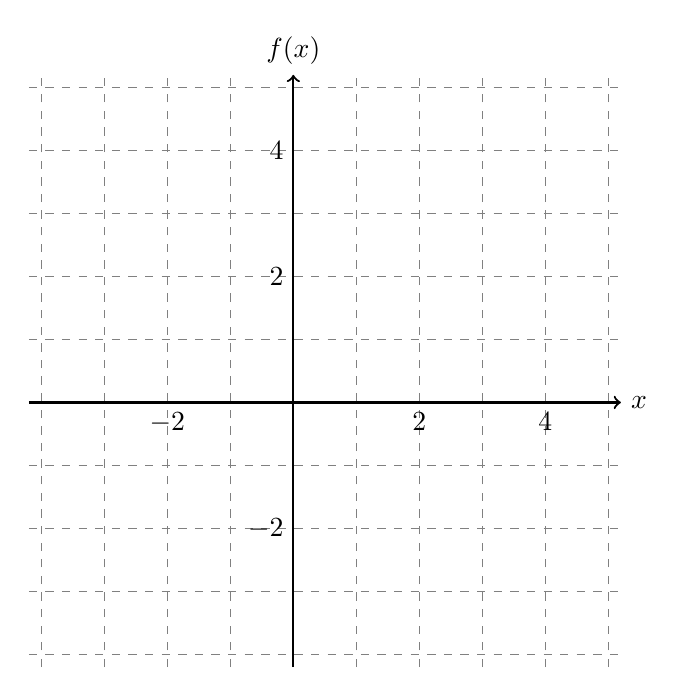
\begin{tikzpicture}[scale=0.8]
\draw [help lines,dashed] (-4.2,-4.2) grid (5.2,5.2);
\draw [thick, ->] (-4.2,0)--(5.2,0) node[right] {$x$};
\draw [thick, ->] (0,-4.2)--(0,5.2) node[above]{$f(x)$};
\foreach \i in {-2,2,4}
{	\node[below] at (\i,0) {$\i$};
}
\foreach \i in {-2,2,4}
{	\node[left] at (0,\i) {$\i$};
}
\end{tikzpicture}
\columnbreak

\begin{subproblems}
\item $f(1)=\emptybox(35pt,25pt)$
\vskip 0.5cm

\item $\d \lim_{x\rightarrow 1^-} f(x)=\emptybox(35pt,25pt)$
\vskip 0.5cm

\item $\d \lim_{x\rightarrow 1} f(x)=\emptybox(35pt,25pt)$
\vskip 0.5cm

\noindent Justify your answer to part \textbf{c}:
\end{subproblems}
\end{multicols}

\problem{4}  Consider the following graph $y=f(x)$.

\begin{minipage}{0.5\textwidth}
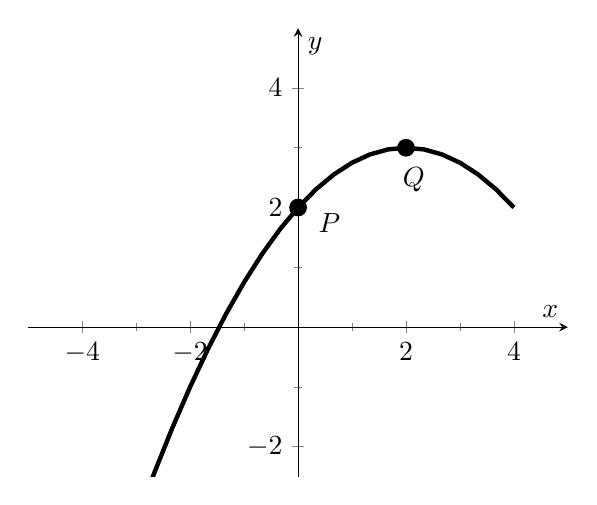
\begin{tikzpicture}
\begin{axis}[scale=1.0, my style,
xtick={-4,-2,...,4}, ytick={-2,0,...,4},
xmin=-5, xmax=5, ymin=-2.5, ymax=5,
minor y tick num=1, minor x tick num=1, mark size=3.0pt]
%
\addplot[domain=-4:4,-,ultra thick] {2 + x - x^2/4};
\addplot[mark=*,only marks] coordinates {(0,2)} node[xshift=4mm,yshift=-2mm] {$P$};
\addplot[mark=*,only marks] coordinates {(2,3)} node[xshift=1mm,yshift=-4mm] {$Q$};
\end{axis}
\end{tikzpicture}
\end{minipage}
\begin{minipage}{0.5\textwidth}
\begin{subproblems}
\item Sketch the secant line through points $P$ and $Q$.  (\textsl{Add the line to the graph at left}.)

\item Find the slope of the secant line through the same points $P(0,2)$ and $Q(2,3)$.
\vskip 4cm

\item Sketch the tangent line through point $P$.
\end{subproblems}
\end{minipage}

\newpage
% compare 2.2 #7,8
\problem{9}
Use the graph of the function $f(x)$ to answer the following questions.
\begin{center}
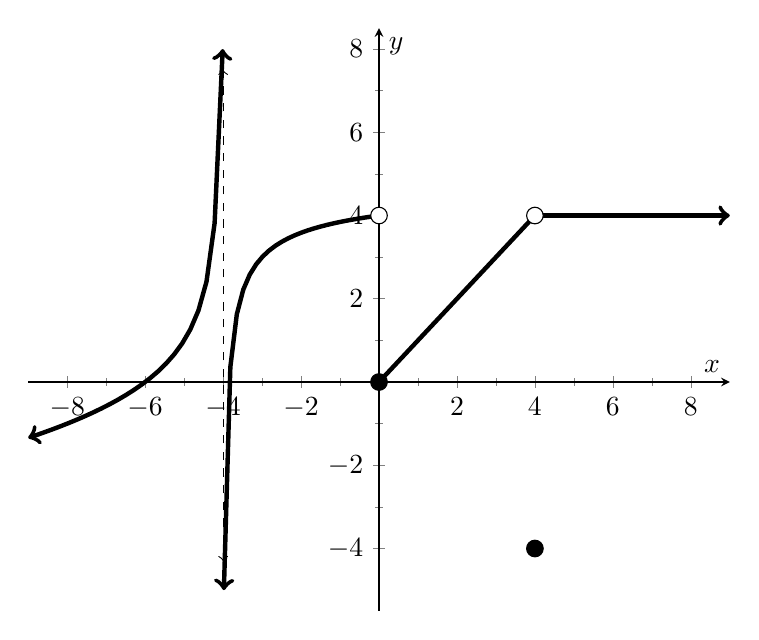
\begin{tikzpicture}
\begin{axis}[scale=1.3, my style,
xtick={-8,-6,...,8}, ytick={-4,-2,...,8},
xmin=-9, xmax=9, ymin=-5.5, ymax=8.5,
minor y tick num=1, minor x tick num=1, mark size=3.0pt]
%
\addplot[domain=-9:-4.01,<->, ultra thick]{min((6+x)/sqrt(-x-4),8)};
\addplot[dashed,<->] coordinates {(-4,-4.3) (-4,7.5)};
\addplot[domain=-3.98:0,<-, ultra thick] {max(5-2/sqrt(((4+x))),-5)};
\addplot[domain=0:4,-,ultra thick] {x};
\addplot[mark=*,only marks] coordinates {(4,-4)(0,0)};
\addplot[mark=*,fill=white,only marks] coordinates {(4,4)(0,4)};
\addplot[domain=4:9,->,ultra thick] {4};
\end{axis}
\end{tikzpicture}
\end{center}

\begin{subproblems}
\begin{multicols}{3}
\item $f(-6)=\mblank{.5in}$
\item $f(0)=\mblank{.5in}$
\item $f(4)=\mblank{.5in}$
\end{multicols}
\begin{multicols}{3}
\item $\d{\lim_{x \to 0^+} f(x)=\mblank{.5in}}$
\item $\d{\lim_{x \to 0^-} f(x)=\mblank{.5in}}$
\item $\d{\lim_{x \to 0} f(x)=\mblank{.5in}}$
\end{multicols}
\begin{multicols}{3}
\item $\d{\lim_{x \to -4^+} f(x)=\mblank{.5in}}$
\item $\d \lim_{x\to 6}f(x)=\mblank{.5in}$
\item $\d{\lim_{x \to 4} f(x)=\mblank{.5in}}$
\end{multicols}
\end{subproblems}

\problem{4} Compute the following limits.
\begin{subproblems}
\item$\d \lim_{x\rightarrow 4} \frac{x-3}{(x-4)^2}=\emptybox(40pt,30pt)$
\vskip 2.5cm

\item$\d \lim_{x\rightarrow 0^+} \frac{2}{\sin(x)}=\emptybox(40pt,30pt)$
\vskip 3cm
\end{subproblems}





\end{document}